\documentclass{tufte-book}
\usepackage[utf8]{inputenc}
\usepackage[english]{babel}
\usepackage{amsmath}
\usepackage{graphicx}
\graphicspath{{../images/}}

\setlength{\parindent}{0pt}

\title{\\ Chemistry \& \\ Materials \\ Science}
\author{Richard Robinson}

\begin{document}
\frontmatter
\maketitle
\tableofcontents

\setlength{\parindent}{0pt}

\mainmatter


%%%%%%%%%%%%%%%%%%%%%%%%%%%%%%%%%%%%%%%%%%%%%%%%%%%%%%%%%%%%%%%%%%%%%%
% MAIN DOCUMENT
%%%%%%%%%%%%%%%%%%%%%%%%%%%%%%%%%%%%%%%%%%%%%%%%%%%%%%%%%%%%%%%%%%%%%%

\chapter{Introduction}

\section{Stoichiometry}

All stoichiometric equations for quantities may be derived from \begin{equation}
  \frac{n_1}{v_1} = \frac{n_2}{v_2}
\end{equation}

\begin{marginfigure}
  \begin{center}
    \begin{tabular}{ll}
      moles & $n = m/M = CV$ \\
      atoms & $n_{\mathrm{atoms}} = \rho V N_a / M$ \\
      molarity & $C = mn/MV$ \\
      dilution & $n_1 = n_2$
    \end{tabular} \phantom{mm}
  \end{center}
  \caption[]{Equations for quantities derived from Equation 1.}
\end{marginfigure}

The percentage yield is defined as \begin{equation}
  \text{\% yield} = \frac{\text{actual yield}}{\text{theo. yield}} \times 100 \%
\end{equation}

A crucial aspect in confirming stoichiometric results is using dimensional analysis; that is, using the dimensions of each unit in the equation(s) and confirming the final unit has the proper dimensions.

\section{Bonding}
The total number of orbitals is equal to $n^2$, where $n$ is the principle quantum number, wherein each orbital has a maximum of two electrons. This maximum occurs only if all subshells contain one electron originally, known as Hund's rule. The orbitals filling order is \begin{equation}
  1s^2 \, 2s^2 \, 2p^6 \, 3s^2 \, 3p^6 \, 4s^2 \, 3d^{10} \, 4p^6 \, 5s^2 \dots
\end{equation}

\begin{fullwidth}
  \begin{center}
    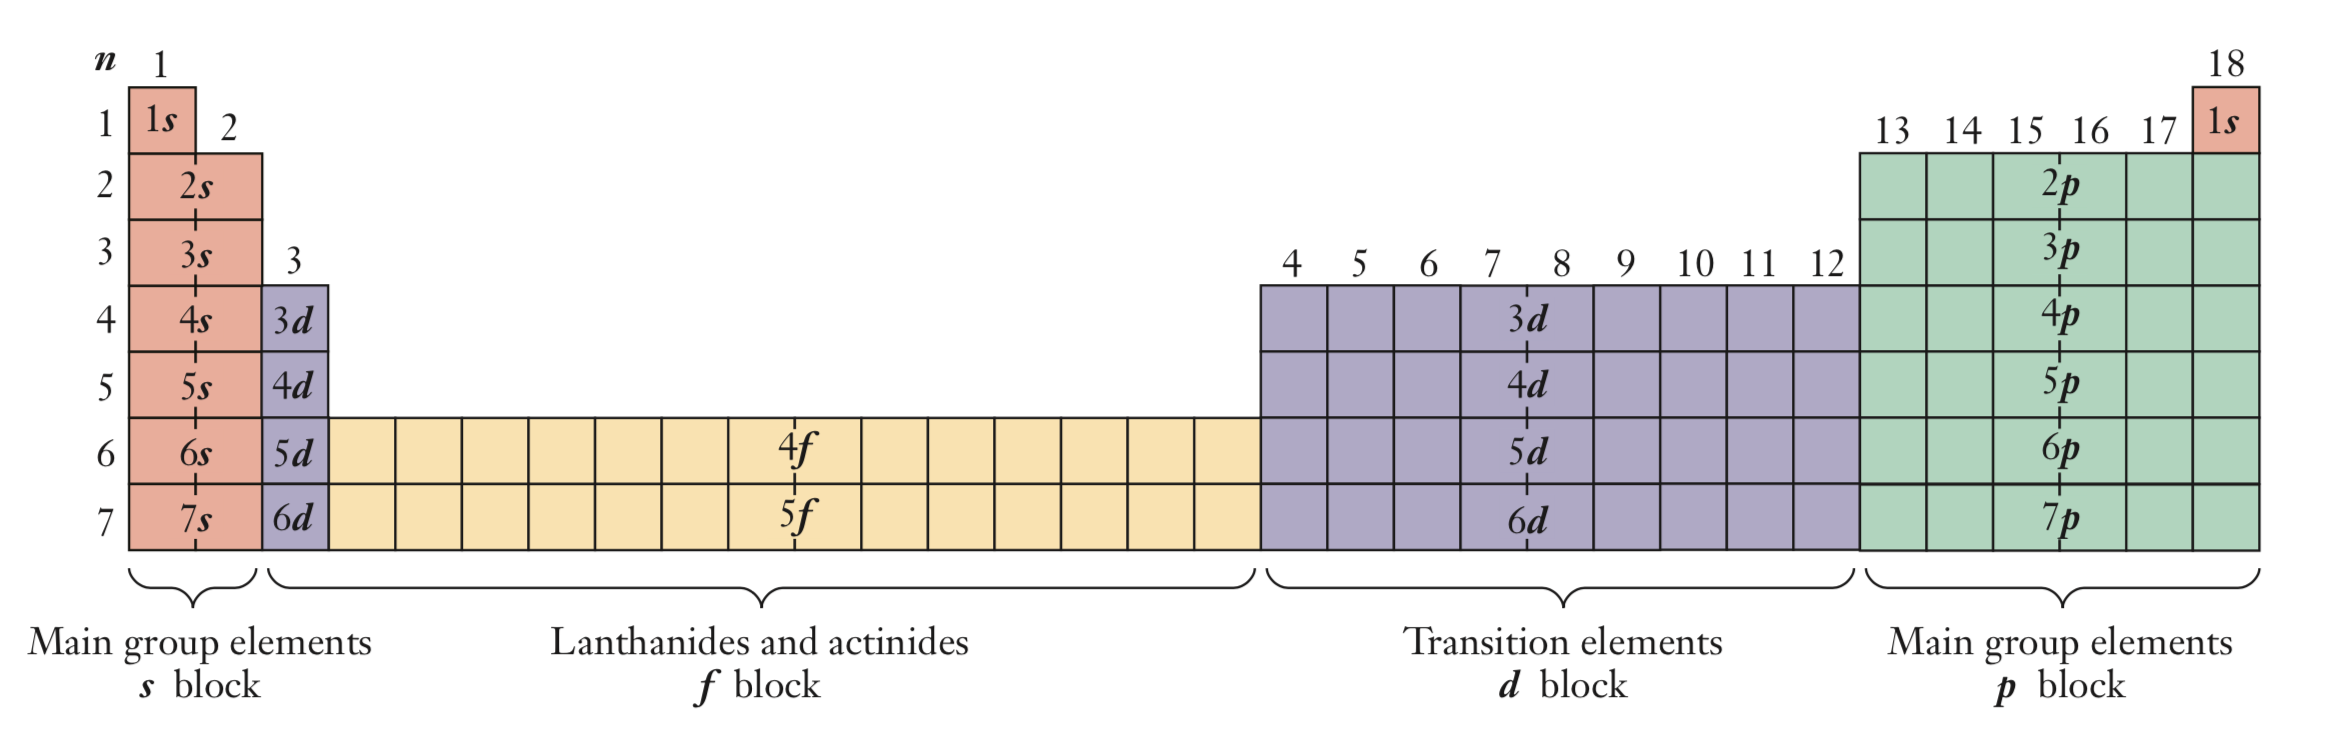
\includegraphics[width=1.5\textwidth]{table}
  \end{center}
\end{fullwidth}

The formal charge is given by $q_f = n_v - n_l - \frac{1}{2} n_s$ in which $\sum q_f = 0$. Hybrid orbitals are dependent 



\end{document}
